\chapter{\label{ch:1-intro}Introduction} 

\minitoc

% TODO 
%{A plan}
% The very first thing to say will be the stuff about light I think, about diagnostic tools essentially always being about controlling the various properties of light (ie electromagnetic waves)

%sections to include
% Start with the laser and our entrance into the multi-petawatt regime with no signs of stopping - ref 40 in Alex Savin's thesis - it looks like that is saying huge growth in laser power check that and maybe write in the thesis but don't include the figure. Also, include a description of CPA and OPCPA
%what is a plasma
%modelling plasma with PIC codes
%intense lasers and absorption mechanisms?? yes for sure but don't do all those just below ZVP
%simulation units and similarity parameter
%Frames of reference - lab, sim, ablating front surface of plasma

% What is the story? Based on the first section by Alex after the abstract
%Plasma is ubiquitous in our known universe and plasma provides us with huge opportunities as a tool to improve our lives
%(From Chen) What we can see in the sky is a result of that stuff being in the plasma state.
%Lasers can do so much now and are only getting more powerful all the time thanks to CPA and since developments (discuss)
%Simulataneously our ability to understand physics has been aided by an explosion in computing power (Peter HEDP paper)
%In this thesis we discuss some of the opportunities that relativistic laser plasma physics offers us with solid density targets - note that note about solids v gases at this point. 
%Perhaps even before the debye length, define what we mean by the temperature of the plasma.

%An unused statement about ion immobility
%Assume for now that the ion-electron mass ratio is infinite, that is to say, the ions are approximately immobile for the timescales under consideration, generally true for a fair few relativistic laser pulse cycles (In later sections the mobility of plasma ions will prove very important but for now this is ignored.).
% I should also discuss ionisation and laser surface plasma interaction./

\section{High-energy-density physics}
We sit on the verge of the exascale revolution both in terms of computing \cite{kotheExascaleComputingUnited2019} and laser power. With rapid adoption of the pioneering advancements of Chirped Pulse Amplification (CPA) by Strickland and Mourou \cite{stricklandCompressionAmplifiedChirped1985} and of Optical Parametric Chirped Pulse Amplification \cite{rossOpticalParametricChirped2000}, multi-petawatt facilities have been commissioned and built across the globe and plans for sub-exawatt facilities are now underway. Figure \ref{fig:intro_lasersystems} details the parameter space accessible by current and proposed facilities \cite{stricklandCompressionAmplifiedChirped1985, fourmauxPedestalCleaningHigh2011, wang085PWLaser2017, tiscarenoOhioStateUniversity2020, sung42PW202017, rossGenerationTerawattPulses2000, yangMultiterawattLaserSystem2002, witte2006source, stoecklHighEnergyPetawattProject2006, lozhkarevCompact56Petawatt2007, herrmannGenerationSubthreecycle162009, andriukaitis90GWPeak2011, zhaoGeneration120GW2013, hoppsOverviewLaserSystems2013, hoppsOverviewLaserSystems2013, thire10MJ5cycle2015, yinHighefficiencyOpticalParametric2016, galesExtremeLightInfrastructure2018, OMEGAFacility, renCompactDoublepassRaman2008, lanciaExperimentalEvidenceShort2010, lanciaSignaturesSelfSimilarRegime2016, marquesJouleLevelHighEfficiencyEnergy2019, thebergeTunableUltrashortLaser2006, trushinSub10fsSupercontinuumRadiation2007, ohIntenseTerahertzGeneration2013, horioGenerationSub17Fs2014, takahashiGeneration10uJCoherent2002, goulielmakisSingleCycleNonlinearOptics2008, skantzakisCoherentContinuumExtreme2009, ferrariHighenergyIsolatedAttosecond2010, takahashiAttosecondNonlinearOptics2013, popmintchevUltravioletSurpriseEfficient2015, nomuraAttosecondPhaseLocking2009, bierbachGeneration10Relativistic2012, heisslerMultimJHarmonicEmission2015, yeungExperimentalObservationAttosecond2017, jahnIntenseIsolatedAttosecond2019, rusEfficientHighbrightnessSoftxray1997, sebbanFullCharacterizationHighgain2000, rusMultimillijouleHighlyCoherent2002, zeitounHighintensityHighlyCoherent2004, wangHighBrightnessInjectionSeededSoftXRayLaser2006, rohringerAtomicInnershellXray2012, ayvazyanFirstOperationFreeelectron2006, ackermannOperationFreeelectronLaser2007, emmaFirstLasingOperation2010, FlashFreeElectronLaser, FlashFreeElectronLaser, FELIXLaboratoryOverview, FELIXLaboratoryOverview, FELIXLaboratoryOverview, kneipObservationSynchrotronRadiation2008, kneipBrightSpatiallyCoherent2010, juEnhancementXraysGenerated2012, chenBrightBetatronXray2013, wangQuasimonoenergeticLaserplasmaAcceleration2013, coleLaserwakefieldAcceleratorsHard2015, wenzQuantitativeXrayPhasecontrast2015, taphuocAllopticalComptonGammaray2012, chenMeVEnergyRaysInverse2013, tsaiCompactTunableCompton2015, polyanskiyPicosecondPulseAmplification2011, haberbergerFifteenTerawattPicosecond2010, glowniaAmplification193nmFemtosecond1992, kandoEnhancementPhotonNumber2009, obenschainHighenergyKryptonFluoride2015, trinesSimulationsEfficientRaman2011, trinesSimulationsEfficientRaman2011, kawanakaConceptualDesignSubexawatt2016, tajimaMarriage20keVSuperconducting2018}, clearly, there is no indication of wavering interest or support for the field of \ac{HED} physics. 
\begin{figure}
	\centering
	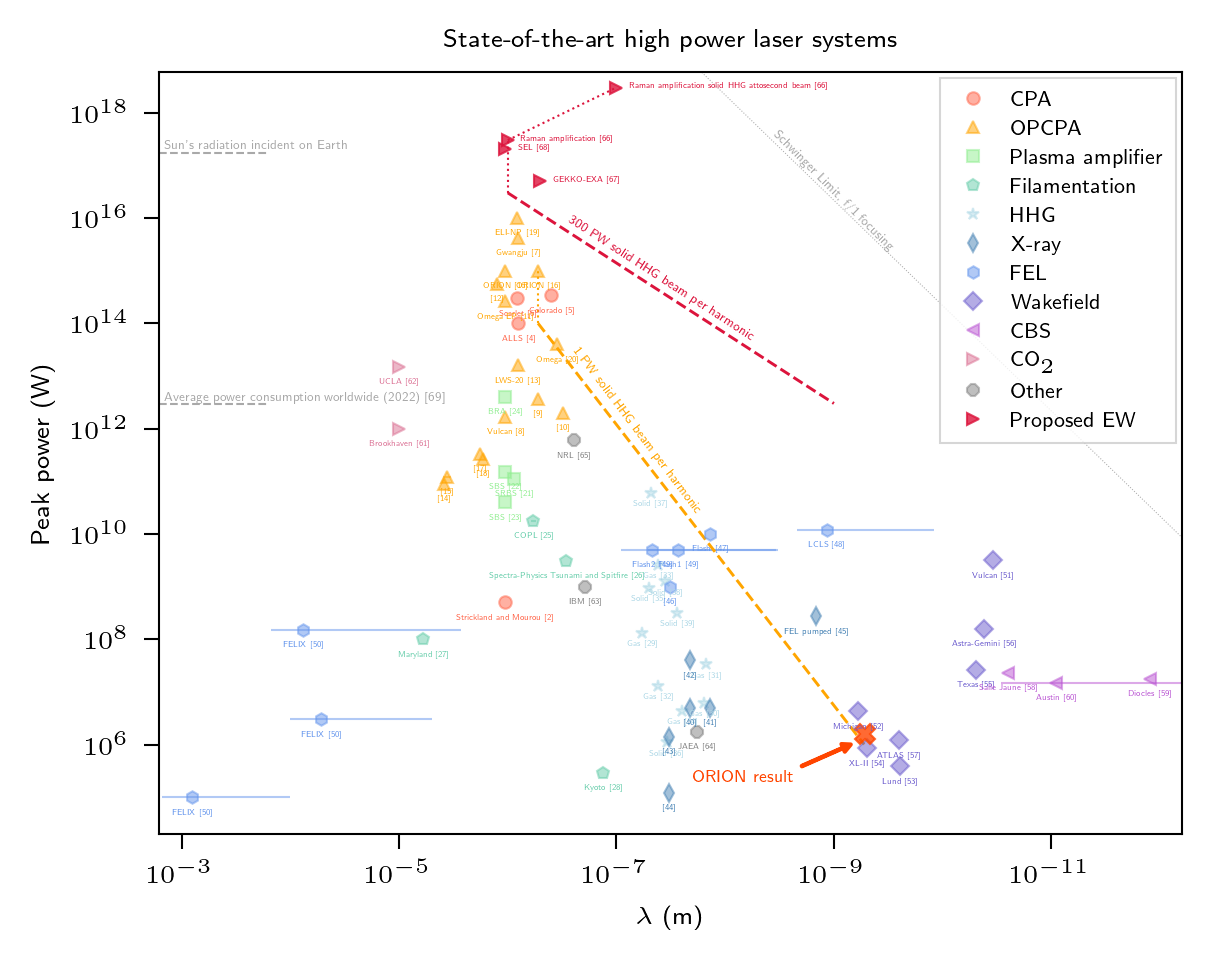
\includegraphics[width=\linewidth]{figures/intro/laser_systems}
	\caption[Laser systems across the globe, both commissioned and theorised.]{A by no means exhaustive plot of laser systems across the globe, both commissioned and theorised \cite{stricklandCompressionAmplifiedChirped1985, fourmauxPedestalCleaningHigh2011, wang085PWLaser2017, tiscarenoOhioStateUniversity2020, sung42PW202017, rossGenerationTerawattPulses2000, yangMultiterawattLaserSystem2002, witte2006source, stoecklHighEnergyPetawattProject2006, lozhkarevCompact56Petawatt2007, herrmannGenerationSubthreecycle162009, andriukaitis90GWPeak2011, zhaoGeneration120GW2013, hoppsOverviewLaserSystems2013, hoppsOverviewLaserSystems2013, thire10MJ5cycle2015, yinHighefficiencyOpticalParametric2016, galesExtremeLightInfrastructure2018, OMEGAFacility, renCompactDoublepassRaman2008, lanciaExperimentalEvidenceShort2010, lanciaSignaturesSelfSimilarRegime2016, marquesJouleLevelHighEfficiencyEnergy2019, thebergeTunableUltrashortLaser2006, trushinSub10fsSupercontinuumRadiation2007, ohIntenseTerahertzGeneration2013, horioGenerationSub17Fs2014, takahashiGeneration10uJCoherent2002, goulielmakisSingleCycleNonlinearOptics2008, skantzakisCoherentContinuumExtreme2009, ferrariHighenergyIsolatedAttosecond2010, takahashiAttosecondNonlinearOptics2013, popmintchevUltravioletSurpriseEfficient2015, nomuraAttosecondPhaseLocking2009, bierbachGeneration10Relativistic2012, heisslerMultimJHarmonicEmission2015, yeungExperimentalObservationAttosecond2017, jahnIntenseIsolatedAttosecond2019, rusEfficientHighbrightnessSoftxray1997, sebbanFullCharacterizationHighgain2000, rusMultimillijouleHighlyCoherent2002, zeitounHighintensityHighlyCoherent2004, wangHighBrightnessInjectionSeededSoftXRayLaser2006, rohringerAtomicInnershellXray2012, ayvazyanFirstOperationFreeelectron2006, ackermannOperationFreeelectronLaser2007, emmaFirstLasingOperation2010, FlashFreeElectronLaser, FlashFreeElectronLaser, FELIXLaboratoryOverview, FELIXLaboratoryOverview, FELIXLaboratoryOverview, kneipObservationSynchrotronRadiation2008, kneipBrightSpatiallyCoherent2010, juEnhancementXraysGenerated2012, chenBrightBetatronXray2013, wangQuasimonoenergeticLaserplasmaAcceleration2013, coleLaserwakefieldAcceleratorsHard2015, wenzQuantitativeXrayPhasecontrast2015, taphuocAllopticalComptonGammaray2012, chenMeVEnergyRaysInverse2013, tsaiCompactTunableCompton2015, polyanskiyPicosecondPulseAmplification2011, haberbergerFifteenTerawattPicosecond2010, glowniaAmplification193nmFemtosecond1992, kandoEnhancementPhotonNumber2009, obenschainHighenergyKryptonFluoride2015, trinesSimulationsEfficientRaman2011, trinesSimulationsEfficientRaman2011, kawanakaConceptualDesignSubexawatt2016, tajimaMarriage20keVSuperconducting2018, NetElectricityConsumption, umstadterRelativisticLaserPlasma2003, dollarEnhancedLaserAbsorption2017} to provide an overview of the parameter space currently and soon to be accessible. The experimental result obtained at the ORION laser facility \cite{hoppsOverviewLaserSystems2013} is presented, and will be discussed in detail in chapter \ref{ch:3-ORION}. The dashed orange line is the accompanying theoretical prediction. The red dashed line indicates the parameter space accessible via the methods discussed in this thesis when coupled with a sub-etawatt Raman amplified laser beam. Such a beam would provide intensities in the water window many orders of magnitude beyond that currently accessible in state-of-the-art facilities. }
	\label{fig:intro_lasersystems}
\end{figure}

\ac{HED} physics is the laboratory study of the behaviour of matter with a pressure above \qty{10}{GPa}, approximately one million atmospheres and containing free electrons not confined to a solid state \cite{drakeFocusHighEnergy2014}, typically in the plasma state of matter. \ac{HED} conditions are found for a vast range of densities and temperatures (from zero to a million million Kelvin) operating in both the quantum and relativistic realms. The applications are equally diverse, including but not limited to inertial confinement fusion, particle acceleration for scientific or medical purposes and light sources for diagnostic tools. Ubiquitous in the natural universe, beyond our solar system, all that can be observed in the sky is radiation emitted from \ac{HED} plasmas \cite{chen}.

This thesis concerns itself with a specific interaction, that of a high-power short-pulse laser incident on a flat solid target. Through the process discussed in this thesis, using state-of-the-art 10 PW laser facilities such as \cite{galesExtremeLightInfrastructure2018}, electron bunches and light pulse of unprecedented charge and brightness can be produced, both with attosecond duration, thus uncovering new avenues for attosecond resolution diagnostics and to access the Schwinger limit. Seemingly counter-intuitively, as the laser power increases, via relativistic effects and for certain conditions, greater coherency in the electron dynamics can be observed and the signals amplified. The red dashed line of figure \ref{fig:intro_lasersystems} could be accessed using next-generation sub-etawatt facilities. Before delving into this fascinating phenomenon, the remainder of this chapter will provide some of the relevant background information. Chapter \ref{ch:2-zvp} introduces the Zero Vector Potential of attosecond absorption in this laser-solid interaction. The following chapter discusses the associated process of Surface High Harmonic Generation and the results of a recent experiment at the ORION laser facility where the absolute intensity of individual X-ray harmonics was measured and compared to the theory.

% TODO reword the intro a little bit. Want to make more of the story. Perhaps discuss the recent Nobel prize and interest in attosecond physics, add an extra line on computing power, and talk about GEMINI.

\section{Electromagnetism fundamentals}
The spatio-temporal propagation of electric $\mathbf{E}(t,\mathbf{x})$ and magnetic $\mathbf{B}(t,\mathbf{x})$ fields must satisfy Maxwell's equations \cite{chenIntroductionPlasmaPhysics2016}
\begin{subequations}
	\label{eq:intro-maxwell}
	\begin{align}
		\nabla \cdot \mathbf{B} &= 0, \label{eq:intro-B0} \\
		\nabla \cdot \mathbf{E} &= \frac{\rho}{\epsilon_0},\label{eq:intro-E0} \\
		\nabla \times \mathbf{B} &= \mu_0 \mathbf{J} + \mu_0 \epsilon_0 \partial_t \mathbf{E},\label{eq:intro-B1} \\
		\nabla \times \mathbf{E} &=-\partial_t \mathbf{B}. \label{eq:intro-E1}
	\end{align}
\end{subequations}
Here, $\epsilon_0 = \qty{8.85e-12}{F.m^{-1}}$ and $\mu_0 = \qty{1.26e-6}{N.A^{-2}}$ are the vacuum permittivity and permeability respectively and $\rho(t,\mathbf{x})$ and $\mathbf{J}(t,\mathbf{x})$ the total charge and current densities of charged particles present. 

A particle with charge $q$ and velocity $\mathbf{v}$ in the presence of electromagnetic fields experiences the Lorentz force,
\begin{equation}\label{eq:intro-Lorentz_force}
	\mathbf{F}_\mathrm{L} = q(\mathbf{E} + \mathbf{v} \times \mathbf{B}).
\end{equation}

The electromagnetic fields can be obtained from the scalar, $\phi$, and vector, $\mathbf{A}$, potentials as  \cite{steaneRelativityMadeRelatively2012}
\begin{equation}
	\mathbf{E} = -\nabla \phi - \partial_t \mathbf{A},
\end{equation}
\begin{equation}
	\mathbf{B} = \nabla \times \mathbf{A}.
\end{equation}

\subsubsection{The Vlasov-Maxwell system of equations}
A collisionless and fully ionised plasma is fully described in the kinetic description by the Vlasov-Maxwell system of equations \cite{derouillatSmileiCollaborativeOpensource2018}. Each plasma species, $s$, of particles with mass $m_s$ and charge $q_s$ is described by its distribution function $f_s(t,\mathbf{x},\mathbf{p})$ at time $t$, position $\mathbf{x}$ and momentum $\mathbf{p} = m_s \gamma \mathbf{v}$. The distribution satisfies the Vlasov equation, that is,
\begin{equation}\label{eq:intro-vlasov}
	(\partial_t + \frac{\mathbf{p}}{m_s\gamma} \cdot \nabla + \mathbf{F}_\mathrm{L} \cdot \nabla_\mathbf{p})f_s = 0,
\end{equation}
where $\mathbf{F}_\mathrm{L}$ is the Lorentz force given in equation \ref{eq:intro-Lorentz_force}. The electric $\mathbf{E}(t,\mathbf{x})$ and magnetic $\mathbf{B}(t,\mathbf{x})$ fields that generate the force must satisfy Maxwell's equations (equations \ref{eq:intro-maxwell}).

This self-consistent system of equations describes the dynamics of plasma particles within electromagnetic fields. The particles modify the fields via their charge and current densities,
\begin{equation}
	\rho(t,\mathbf{x}) = \sum_s q_s \int d^3pf_s(t,\mathbf{x},\mathbf{p}),
\end{equation}
and 
\begin{equation}
	\mathbf{J}(t,\mathbf{x}) = \sum_s q_s \int d^3p\mathbf{v}f_s(t,\mathbf{x},\mathbf{p}),
\end{equation}
respectively.

\section{\label{sec:plasma_def}The definition of a classical plasma}
As outlined in F. Chen's definitive textbook `Introduction to Plasma Physics and Controlled Fusion' \cite{chenIntroductionPlasmaPhysics2016}, a plasma must fulfil three criteria, namely,
% TODO make a note that in a quantum plasma, one does not want lots of particles in the Debye sphere

\begin{enumerate}
	\item Ionisation: a plasma must consist of both charged and neutral particles, of course, this alone cannot define a plasma, any gas will contain some degree of ionisation, however, with reference to figure \ref{fig:intro_lasersystems}, clearly, modern high power laser systems will instantaneously fully ionise a target upon incidence;
	\item Quasineutrality: while locally there can be (often extreme) electromagnetic forces and charge concentrations at work, over the length scales of the plasma, such forces are screened out and the plasma bulk remains net neutral in charge;
	\item Collective behaviour: unlike in a gas, where collisions will dominate the dynamics, the particles in a plasma generate electromagnetic fields that interact at a distance and thus a particle's motion depends not only on its immediate vicinity but on the surrounding plasma conditions, indeed often it is the so-called \textit{collisionless} plasmas where collisions can be safely neglected that are of most interest, as is the focus of this thesis.
\end{enumerate}

These conditions can be quantitatively described by the Debye length, the plasma parameter and the plasma frequency as laid out in the following sections.

\subsection{\label{sec:debye_length}The Debye length}
The Debye length describes the extent to which a plasma can shield electromagnetic fields within and so remain quasineutral. Consider an infinitely extending plasma with a test charge placed at some point, then what would be the scalar potential $\phi(\mathbf{x})$ around it? If the plasma had no kinetic energy, the charged particles would arrange themself immediately adjacent to the test charge and once this equilibrium state was reached there would be no electromagnetic fields present. More realistically, the plasma will have some temperature, likely a very large temperature and so some particles will be able to escape the potential of the test charge and thus leak electromagnetic fields into the plasma bulk. Poisson's equation (equation \ref{eq:intro-E0} in the static case) reads
\begin{equation}\label{eq:poisson}
	\epsilon_0\nabla^2\phi = -e(Zn_\mathrm{i} - n_\mathrm{e}),
\end{equation}
where $\epsilon_0 = \qty{8.854e-12}{F.m^{-1}}$ is the permittivity of free space, $e = \qty{1.602e-19}{C}$ is the charge of an electron, $Z$ is the plasma ion charge in units of $e$ and $n_\mathrm{i}$ and $n_\mathrm{e}$ are the number densities of plasma ions and electrons.

Since the electrons are significantly more mobile than the ions due to their lower mass, it is in general the electrons and not the ions that respond to the test charge and the ions can be assumed to provide a constant background of positive charge density.
If the number density of electrons follows a Boltzmann temperature distribution in the presence of a potential energy $-e\phi$, then
\begin{equation}\label{eq:nj_boltzmann}
	n_\mathrm{e}= n_{\mathrm{e},0}e^{e\phi/KT_\mathrm{e}},
\end{equation}
where $n_{\mathrm{e},0}$ is the electron number density far from the test charge, $n_\mathrm{i} = n_{\mathrm{e},0}/Z$, $K = \qty{1.38e-23}{J.K^{-1}}$ is the Boltzmann constant and $T_\mathrm{e}$ is the electron temperature in Kelvin. Note that in plasmas it is very common for different species to have differing temperatures depending on the mechanism for energy absorption and the timescales for collisions compared to the timescale of the study.

Substituting equation \ref{eq:nj_boltzmann} into equation \ref{eq:poisson} and Taylor expanding the exponential term in the limit that the plasma is weakly coupled ($e\phi << KT_\mathrm{e}$), 
\begin{equation}\label{eq:poisson_debye2}
	\nabla^2\phi = \frac{\phi}{\lambda_\mathrm{D}^2},
\end{equation}
where
\begin{equation}\label{eq:debye}
	\lambda_\mathrm{D} \equiv \sqrt{\frac{\epsilon_0KT_\mathrm{e}}{n_\mathrm{e}e^2}},
\end{equation}
is the \textit{Debye length} and describes the thickness of the charge sheath surrounding the test charge. For quasineutrality to hold for the plasma bulk, its spatial dimensions, $L$, must extend beyond a few Debye lengths, \textit{i.e.}
\begin{equation}
	L \gg \lambda_D.
\end{equation}

\subsection{\label{sec:plasma_parameter}The plasma parameter}
In order for the derivation of section \ref{sec:debye_length} to be statistically valid, there must be a large number of charged particles within the shielding sheath. The number of particles within the \textit{Debye sphere} is
\begin{equation}\label{eq:plasma_parameter}
	N_\mathrm{D} = \frac{4}{3}\pi\lambda_\mathrm{D}^3n,
\end{equation}
where, $N_\mathrm{D}$ is the \textit{plasma parameter}. Note that, as discussed above, in most cases it is most suitable to choose the number density $n$ to be the number density of electrons, $n_\mathrm{e}$. To ensure the plasma is suitably ionised (criterion 1) and that the plasma engages in collective behaviour (criterion 3),
\begin{equation}\label{eq:plasma_parameter_condition}
	N_\mathrm{D} \ggg 1.
\end{equation}
\subsection{\label{sec:plasma_frequency}Collisionality and the plasma frequency}
Collective behaviour not only depends on the ability for large numbers of particles to interact via electromagnetic forces but also that these forces dominate over collisions in describing particle trajectories. Taking $\omega$ as the typical frequency of plasma oscillations and $\tau$ as the average time between collisions, for a plasma (as opposed to a gas)
\begin{equation}\label{eq:plasma_frequency_condition}
	\omega\tau > 1
\end{equation}
is required. It now remains to determine what is the typical frequency of collisions in a given plasma. While the types of plasma waves and their associated frequencies of oscillation are multitudinous, the characteristic frequency, the \textit{plasma frequency}, $\omega_\mathrm{p}$, is the most straightforward. It describes the response of electrons to charge imbalances within an infinite uniform plasma at rest in the absence of magnetic fields or temperature fluctuations. As noted in section \ref{sec:debye_length}, the ions provide a constant background of positive charge.

Consider a semi-infinite plasma existing for $x>0$, with electron density $n_\mathrm{e}$ and ion density $n_\mathrm{e}/Z$ of charge state $Z$\footnote{This description has direct relevance to the Zero Vector Potential mechanism which will be made clear in chapter \ref{ch:2-zvp}.}. Suppose the electron fluid is displaced by some perfectly isotropic force into the plasma bulk a distance $(\Delta x) \hat{\mathbf{x}}$ as in figure \ref{fig:introplasmafrequency}. 
\begin{figure}
	\centering
	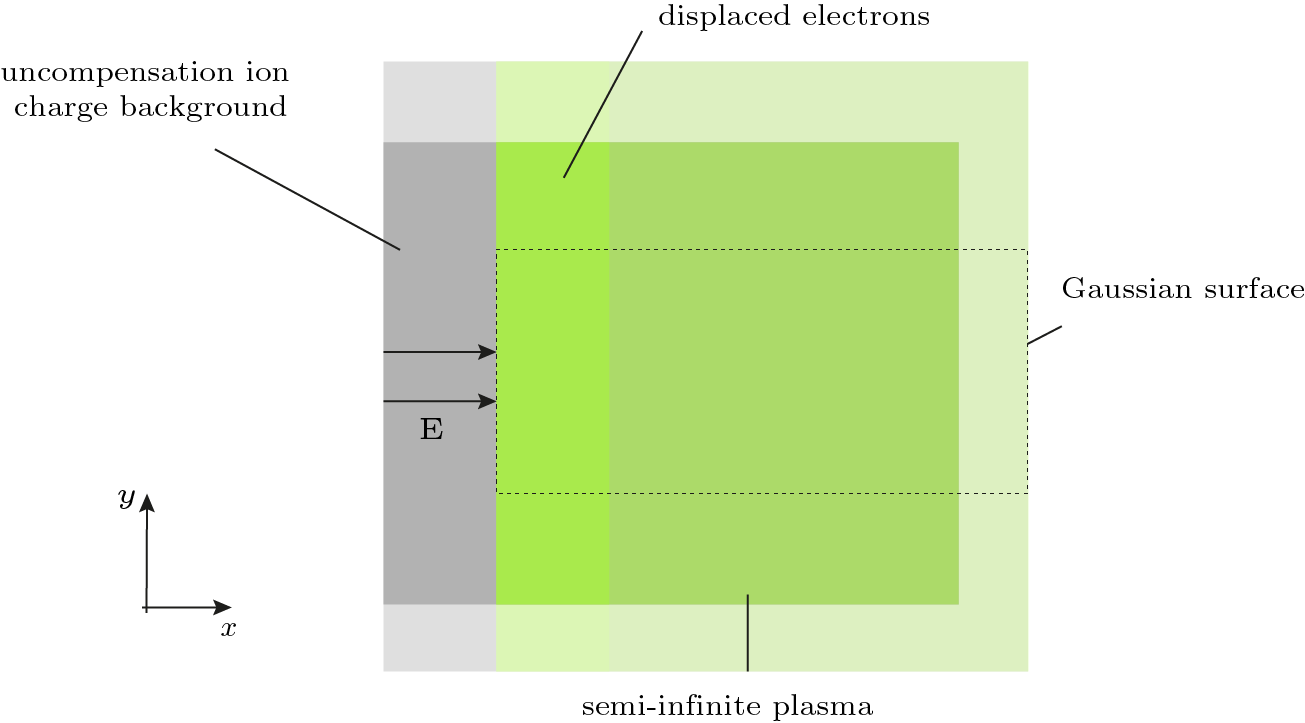
\includegraphics[width=0.7\linewidth]{figures/intro/intro_plasma_frequency}
	\caption[Diagram to illustrate the derivation of the plasma frequency.]{The electrons of a semi-infinite plasma are displaced inwards by some external force leaving in their wake an uncompensated space charge of `immobile' positive ions. By constructing a Gaussian surface along the dashed line, using Gauss' Law, the electric field associated with the positive space charge can be calculated.}
	\label{fig:introplasmafrequency}
\end{figure}
The total charge of displaced electrons within a surface area of $\sigma$ is 
\begin{equation}\label{eq:intro_Q}
	Q = -en_\mathrm{e}\sigma\Delta x.
\end{equation}
Applying the integral form of Gauss' law (from equation \ref{eq:intro-E0}) to the surface detailed in figure \ref{fig:introplasmafrequency}, the uncompensated charge leads to 
\begin{equation}\label{eq:intro_E}
	-\sigma E\hat{\mathbf{x}}= \frac{Q}{\epsilon_0}\hat{\mathbf{x}} = -\frac{en_\mathrm{e}\sigma\Delta x}{\epsilon_0}\hat{\mathbf{x}}
\end{equation}
at the electron surface. By the Lorentz force, equation \ref{eq:intro-Lorentz_force}, the displaced electrons will experience a restoring force, $-eE\hat{\mathbf{x}}$, perpendicular to the surface due to the electron-ion charge imbalance. The equation of motion for electrons on that surface is therefore
\begin{equation}\label{eq:intro_sho}
	m_e\frac{\mathrm{d}^2\Delta x}{\mathrm{d}t^2} = -eE = -\frac{e^2n_\mathrm{e}}{\epsilon_0}\Delta x.
\end{equation}
Equation \ref{eq:intro_sho} clearly describes a simple harmonic oscillator with a characteristic frequency given by the plasma frequency,
\begin{equation}
	\omega_\mathrm{p} = \sqrt{\frac{e^2n_\mathrm{e}}{m_\mathrm{e} \epsilon_0}}.
\end{equation}

% TODO Scheck's notes cover that the collisionality condition is always satisfied for a classical plasma (Archie Bott to send the notes)

\section{The Lawson-Woodward theorem}\label{sec:intro-lawson_woodward}
The Lawson-Woodward theorem states that there can be no net electron energy gain using laser fields \cite{esareyPhysicsLaserdrivenPlasmabased2009}, quite at odds with one of the primary aims of this thesis, that is, the acceleration of electrons. There are, however, several conditions that must be met, namely,
\begin{enumerate}
	\item The interaction region is infinite;
	\item The interaction  occurs in a vacuum;
	\item The electron is ultra-relativistic ($v\approx c$) along the acceleration gradient;
	\item No electro- or magnetostatic fields are present;
	\item Non-linear effects are neglected.
\end{enumerate}
Several of these will be applicable to the various accelerations of electrons considered. It is this final condition that is most damning to the application of the theorem. Throughout this thesis, the ultra-relativistic laser pulses under consideration ensure non-linear effects cannot be neglected. It is indeed such non-linearities that are of most interest.


\section{Laser-solid density plasma linear interaction}\label{sec:intro-lasersolidplasma_linear}
Consider small transverse electromagnetic waves propagating through a plasma. Linearising equation \ref{eq:intro-Lorentz_force} for a single plasma electron by assuming only small field variations and thus small velocity variation,
\begin{equation}\label{eq:intro-EOM_linear}
	m_\mathrm{e}  \dot{\mathbf{v}}_\mathrm{e} = -e\mathbf{E}.
\end{equation}
Combining the time derivative of equation \ref{eq:intro-B1} and the curl of equation \ref{eq:intro-E1},
\begin{equation}
	\nabla\times\nabla \times \mathbf{E}= - \mu_0 \dot{\mathbf{J} }- \mu_0\epsilon_0 \ddot{\mathbf{E}}.
\end{equation}
Considering only fast oscillations such that ions are effectively immobile,
\begin{equation}
	\mathbf{J} = - n_\mathrm{e} e\mathbf{v}_\mathrm{e}
\end{equation}
and using the identity $\nabla\times\nabla \times \mathbf{E} = \nabla(\nabla\cdot \mathbf{E}) - \nabla^2\mathbf{E}$,
\begin{equation}
	\nabla(\nabla\cdot \mathbf{E}) - \nabla^2\mathbf{E} = -\frac{\mu_0 n_\mathrm{e} e^2}{m_\mathrm{e}} \mathbf{E}  - \mu_0 \epsilon_0 \ddot{\mathbf{E}}.
\end{equation} 
Assuming plane wave solutions of the form
\begin{equation}
	\mathbf{E} = \mathbf{E_0}e^{i(\mathbf{k}\cdot \mathbf{x}-\omega t)},
\end{equation}
where $\mathbf{k}$ is the wave-vector and $\omega$ the frequency of oscillations and noting the waves are transverse $\mathbf{k}\cdot \mathbf{E} = 0$,
\begin{equation}
	|\mathbf{k}|^2 \mathbf{E} = -\frac{\mu_0 n_\mathrm{e} e^2}{m_\mathrm{e}}\mathbf{E} + \mu_0\epsilon_0\omega^2\mathbf{E}
\end{equation}
and hence the dispersion relation for electromagnetic waves propagating in a plasma is
\begin{equation}\label{eq:intro-EM_dispersion}
	\omega^2  = c^2|\mathbf{k}|^2  + \omega_\mathrm{p}^2.
\end{equation}
Equation \ref{eq:intro-EM_dispersion} exhibits a \textit{cutoff} dependent on the plasma density via $\omega_\mathrm{p}$. The \textit{critical density}, $n_\mathrm{c}$, is defined as the density above which a laser pulse of frequency $\omega_\mathrm{L}$ cannot propagate through a plasma. This occurs for $\omega_\mathrm{L} = \omega_\mathrm{p}$, thus,
\begin{equation}
	n_\mathrm{c} = \frac{m_\mathrm{e}\epsilon_0 \omega_\mathrm{L}^2}{e^2}.
\end{equation}
As the plane wave has a spatial dependence $\sim \exp{(\mathbf{k}\cdot\mathbf{x})}$, if $n_\mathrm{e} > n_\mathrm{c}$, $\mathbf{k}$ is imaginary and the wave no longer propagates through the plasma and instead exponentially attenuates over a skin depth,
\begin{equation}
	\delta = \frac{1}{|\mathbf{k}|} = \frac{c}{\sqrt{\omega_\mathrm{p}^2 - \omega_\mathrm{L}^2}}
\end{equation}
and is reflected. For typical high-power lasers with wavelengths in the visible or near-infrared, fully ionised solids tend to have densities well above the critical density and thus 

\section{Relativity}
Modern high-power lasers operate in the domain of relativistic mechanics and in general interactions are highly non-linear. It is useful to introduce some of the basic principles of relativity. Note that while there has been growing interest in the curvature of spacetime by relativistic lasers \cite{atongaGravitationalWavesHighpower2023}, this effect remains undetectable at present. Thus, throughout this thesis, the inner product of 4-tensors is defined using the Minkowski Metric \cite{steaneRelativityMadeRelatively2012}. 

Many useful quantities can be arranged into contravariant four-vectors that undergo a Lorentz transformation for a change of frame of reference \cite{steaneRelativityMadeRelatively2012}, specifically, 
\begin{equation}
	\mathbf{A}'^\mu =\Lambda_\mu^\nu \mathbf{A}^\mu,
\end{equation}
where $\Lambda^\mu_\nu$ is the appropriate Lorentz transformation, and primed symbols typically denote boosted frames of reference. Without loss of generality, the coordinate system can be defined such that the boosted frame travels along the $\mathbf{x}$-axis with respect to the initial frame. Thus, the Lorentz transformation is defined
\begin{equation}\label{eq:zvp_lorentz}
	\Lambda_\mu^\nu = \begin{pmatrix}
		\gamma & -\beta\gamma & 0 & 0\\
		-\beta\gamma & \gamma & 0 & 0\\
		0 & 0& 1 & 0\\
		0 & 0 & 0 & 1
	\end{pmatrix}.
\end{equation}
Generally, a \textit{beta factor} is a normalised speed or velocity of an object,
\begin{equation}
	\beta = \frac{v}{c}, 
\end{equation}
here it refers to the frame velocity and its associated Lorentz or \textit{gamma factor} is
\begin{equation}
	\gamma = \frac{1}{\sqrt{1-\beta^2}}.
\end{equation}
Four-vectors relevant to this thesis are listed in table \ref{tab:intro-four-vectors}.
%Many useful quantities can be arranged into contravariant four-vectors that undergo a Lorentz transformation for a change of frame of reference, those relevant to this thesis are: the four-displacement
%\begin{equation}
%	\mathbf{X}^\mu = (ct, \mathbf{x}),
%\end{equation}
%the four-potential
%\begin{equation}
%\mathbf{A}^\mu = \left(\frac{\phi}{c}, \mathbf{A}\right),
%\end{equation}
%the four-current density
%\begin{equation}
%	\mathbf{J}^\mu = (c\rho,\mathbf{J}),
%\end{equation}
%the four-wave vector
%\begin{equation}
%	\mathbf{K}^\mu = \left(\frac{\omega}{c}, \mathbf{k}\right)
%\end{equation}
%and the four-momentum of a particle
%\begin{equation}
%	\mathbf{P}^\mu = \left(\frac{U}{c}, \mathbf{p}\right),
%\end{equation}
%where $U = \gamma m c^2$ is the particle energy and $\mathbf{p} = \gamma m\mathbf{v}$ its three-momentum.
\begin{table}
	\begin{center}
		\begin{tabular}{llll}
			\hline \hline
			Symbol & Name & Components & Invariant \\
			\hline
			$\mathbf{X}^\mu$& 4-displacement & $(ct, \mathbf{x})$ & $-c^2\tau^2$  \\
			$\mathbf{A}^\mu$&4-potential  & $(\phi/c, \mathbf{A})$  &  \\
			$\mathbf{J}^\mu$& 4-current density & $(c\rho,\mathbf{J})$ & $-c^2\rho_0^2$ \\
			$\mathbf{K}^\mu$& 4-wave vector &$(\omega/c, \mathbf{K})$  &  \\
			$\mathbf{P}^\mu$& 4-momentum &  $(U/c, \mathbf{p})$& $-m^2c^2$ \\
			\hline \hline
		\end{tabular}
		\caption{\label{tab:intro-four-vectors} Four-vectors of relevance to this thesis. New parameters are the proper time, $\tau$, the proper charge density, $\rho_0$, energy, $U = \gamma m c^2$, three-momentum, $p = \gamma m\mathbf{v}$.}
	\end{center}
\end{table}
Transformations of electromagnetic fields under reference frame boosts are given in appendix \ref{sec:app_lorentzEM} and Maxwell's equations are Lorentz covariant.

Focusing now on the 4-potential $\mathbf{A}^\mu$, choosing the Lorenz gauge,
\begin{equation}
	\partial_\mu \mathbf{A}^\mu = \nabla \cdot \mathbf{A} + \frac{1}{c^2}\partial_t \phi = 0,
\end{equation}
then Maxwell's equations can be written
\begin{equation}\label{eq:intro-wave_equation}
	\partial_\nu \partial^\nu \mathbf{A}^\mu = -\frac{1}{c^2\epsilon_0}\mathbf{J}^\mu.
\end{equation}
Equation \ref{eq:intro-wave_equation} can then be solved to yield 
\begin{equation}
	\mathbf{A}(\mathbf{x},t) = \frac{\mu_0}{4\pi} \int \frac{\mathbf{J}(\mathbf{x'},t_\mathrm{a})}{|\mathbf{x}-\mathbf{x}'|} \mathrm{d}^3\mathbf{x}',
\end{equation}
where $t_\mathrm{a} = t- |\mathbf{x}-\mathbf{x}'|/c$ is the advanced time.

\subsection{Ultra-relativistic similarity theory}
Consider a relativistically intense laser pulse normally incident on a collisionless plasma as in figure \ref{fig:introplasmafrequency} and neglect ion motion. The electron distribution is fully described by the Vlasov equation (equation \ref{eq:intro-vlasov}) with the self-consistent electric and magnetic fields satisfying Maxwell's equations (equations \ref{eq:intro-maxwell}). Suppose the incident laser pulse has an initial vector potential 
\begin{equation}
	\mathbf{A}(t=0) = \mathbf{a}((y^2+z^2)/R^2,x/c\tau)\cos k_\mathrm{L}x.
\end{equation}
This envelope form for the potential, $\mathbf{a}((y^2+z^2)/R^2,x/c\tau)$, is sensible provided $k_\mathrm{L}R \gg 1$ and $\omega_\mathrm{L}\tau \gg 1$, where $R$ is the focal spot radius and $\tau$ the pulse duration. For fixed laser envelope, the laser-plasma dynamics depend on just four dimensionless variables:  the normalised focal spot size, $k_\mathrm{L} R$, the normalised pulse duration, $\omega_\mathrm{L}\tau$, the normalised laser vector potential amplitude
\begin{equation}
	a_0 = \mathrm{max}\left|\frac{e \mathbf{a} }{m_\mathrm{e} c^2 }\right|,
\end{equation}
in terms of the peak laser electric field amplitude $\mathbf{E}_\mathrm{L}$,
\begin{equation}
	a_0 = \frac{e|\mathbf{E}_\mathrm{L}|}{m_\mathrm{e} c\omega_\mathrm{L}},
\end{equation}
and the normalised plasma density
\begin{equation}
	\bar{n}_\mathrm{e} = \frac{n_\mathrm{e}}{n_\mathrm{c}}.
\end{equation}
By normalising the system of equations, details given in the appendix, and combining these last two expressions into the \textit{relativistic similarity parameter},
\begin{equation}
	S = \frac{\bar{n}_\mathrm{e}}{a_0},
\end{equation}
it is possible to show that in the ultra-relativistic limit ($a_0 \gg 1$), the dynamics of the system are similar for constant $S$ \cite{gordienkoScalingsUltrarelativisticLaser2005} with plasma electrons following similar trajectories where 
\begin{equation}\label{eq:intro-p_similarity}
	\mathbf{p} \sim a_0.
\end{equation}
There is also a more physical meaning to the $S$ parameter. Consider again section \ref{sec:intro-lasersolidplasma_linear} on the propagation of linear electromagnetic waves through a plasma but now for the case of an ultra-relativistic laser pulse. For an electron rotating in an electromagnetic field,
\begin{equation}
	\mathbf{F}_\perp = \gamma m_e \mathbf{a}_\perp,
\end{equation}
where $ \mathbf{a}_\perp$ is the acceleration perpendicular to the motion and thus the response of the electrons is reduced by a factor of $\gamma$. While some find the \textit{relativistic mass} correction to be somewhat unhelpful nomenclature for the phenomenon \cite{steaneRelativityMadeRelatively2012}, it has nevertheless become commonplace within the literature of relativistic plasma physics \cite{umstadterRelativisticLaserPlasma2003}. Turning the handle, one finds that the relativistic plasma frequency is
\begin{equation}
	\omega_\mathrm{p}^\mathrm{rel} = \sqrt{\frac{e^2n_\mathrm{e}}{\gamma m_\mathrm{e} \epsilon_0}}.
\end{equation}
Using equation \ref{eq:intro-p_similarity}, and taking $v \approx c$, then $\gamma \approx a_0$ and the normalised relativistic cutoff density is simply $S$. Thus, the ultra-relativistic similarity parameter is just a measure of the overdensity of a plasma once relativistic corrections have been applied, \textit{i.e.} for $S>1$, a laser pulse will be reflection, however for $\bar{n}_\mathrm{e} > 1$ and $S <1$, one enters the regime of relativistically self-induced transparency \cite{ereminRelativisticSelfInducedTransparency2010}. It is now possible to define the parameter space of interest in this thesis: relativistic laser-plasma surface interactions occur for $a_0 \gg 1$ and $S > 1$.

\subsection{Relativistic lasers and plasmas}
The descriptor \textit{relativistic} is applied liberally in this thesis. When applied to electromagnetic fields or laser pulses it refers to 
\begin{equation}
	a_0 \ge 1.
\end{equation}
When applied to particles, their Lorentz factors are
\begin{equation}
	\gamma = \frac{1}{\sqrt{1-\beta^2}} \ge 2,
\end{equation}
corresponding to a speed, $u \ge 0.87 c$. \textit{Ultra-relativistic} implies these quantities are much larger than the conditions provided. A relativistic laser pulse will accelerate electrons to relativistic velocities in a fraction of a laser pulse cycle. Consider an electron in the presence of a uniform electric field of magnitude $a_0 = 100$, an intensity accessible by current state-of-the-art laser facilities. The work done on that particle by the field is 
\begin{equation}
	T = (\gamma -1)m_\mathrm{e}c^2 = \int \mathbf{E}\cdot \mathrm{d} \mathbf{x},
\end{equation}
The field will accelerate an electron to relativistic velocities in a distance less than 1 \% of a corresponding laser pulse wavelength.

Upon entrance to the relativistic regime, the motion of an electron fundamentally changes. Consider Equation \ref{eq:intro-Lorentz_force}. For non-relativistic laser pulses, the magnetic field component can be neglected and the electron will simply oscillate along the electric field vector direction. Once electron velocities approach $c$, this approximation is no longer valid, electron velocities are rotated in the magnetic field and are accelerated along the laser propagation direction. In a plasma, this enables compression of a surface since ions are accelerated inwards in longitudinal electric fields from the induced electron-ion separation.

\subsection{Conservation of generalised transverse momentum}\label{sec:intro_conservation-generalised-mometum}
Consider a holonomic system of $N$ relativistic particles under the influence of electromagnetic forces. A particle $j$ with charge $e_j$ and mass $m_j$ experiences a scalar potential,
\begin{equation}
	V_{j} = e_j(\phi - \mathbf{A} \cdot \mathbf{v}_{j})
\end{equation}
and hence the system is described by the Lagrangian \cite{goldsteinClassicalMechanics2013}
\begin{equation}
	\mathcal{L} = \sum^N_{j=1}\left( - m_jc^2\sqrt{1-\beta^2_\mathrm{j}} - e_j(\phi - \mathbf{A} \cdot \mathbf{v}_j) \right),
\end{equation}
The generalised momentum corresponding to coordinate $x_j$ is
\begin{equation}
	p_{j,x} = \frac{\partial L}{\partial \dot{x}_j} = \frac{m_j\dot{x}_j }{\gamma_j}+ e_jA_x,
\end{equation}
thus, the generalised momentum describes both the linear mechanical momentum and the momentum of the electromagnetic field. Via Noether's theorem, if $L$ is independent of $x_j$, \textit{i.e.} spatially homogeneous along $x$ for particle $j$, then 
\begin{equation}\label{eq:intro-transverse_momentum_differential_equation}
	\dot{p}_{j,x} = 0
\end{equation}
since
\begin{equation}
	\frac{\mathrm{d}}{\mathrm{d}t}\left(\frac{\partial L}{\partial \dot{x}_j}\right) = \frac{\partial L}{\partial x_j}.
\end{equation}

Taking the Lorenz gauge, consider a linearly polarised Gaussian laser pulse, with an axis of polarisation along $x$ incident on a solid target at rest. Then $A_x$ is approximately constant along $x$ near the beam centre\footnote{Constant relative to the scale of typical electron trajectories in such an interaction.}. Integrating equation \ref{eq:intro-transverse_momentum_differential_equation}, fully constraining the gauge by setting the potential to zero initially, and noting that there is no linear momentum at the target, the generalised transverse momentum conservation equation for an electron in the laser field is
\begin{equation}\label{eq:intro-transverse_momentum_conservation_no_initial_momentum}
	p_\mathrm{T} = eA,
\end{equation}
where $p_\mathrm{T}$ is the electron momentum along the polarisation axis of the laser pulse and $A$ is the laser pulse 3-vector potential amplitude. As a sanity check, this expression complies with the ultra-relativistic similarity result of equation \ref{eq:intro-p_similarity}.
% TODO note that setting the boundary conditions is the final requirement to fix the gauge in the Lorenz gauge formalism.


Note that this is only valid provided the electron does not radiate along the direction of polarisation as discussed by Sokolov \textit{et al} \cite{sokolovDynamicsEmittingElectrons2009}. The implications of \textit{Radiation Reaction }are discussed in the following section.

\section{QED effects}
% TODO cite Schwinger limit
Next-generation laser facilities will enable the testing of decades-old theoretical predictions of \ac{SF-QED}. Already Fedeli \textit{et al} have shown in simulations that current PW-class laser facilities can access the regime using an all-optical set-up based on laser-solid surface interactions \cite{fedeliProbingStrongfieldQED2020}. The Schwinger Limit $E_\mathrm{S} = \qty{1.32e18}{V.m^{-1}}$ is the field intensity at which the vacuum becomes non-linear. If by some means an electron can be directed towards a plane electromagnetic wave, by consideration of the Lorentz transformations of electromagnetic fields (equations \ref{eq:app-maxwell_transformation}), it is possible that provided the electron is sufficiently relativistic, in its own frame of rest it will `see' electromagnetic fields intense enough to access vacuum non-linearities. The first two frontiers of SF-QED that will be accessible are Radiation Reaction and multi-photon Breit-Wheeler electron pair production. Brief introductions to these phenomena are now presented.

\subsection{High-energy photon emission and radiation reaction}
When a charged particle undergoes an acceleration, it emits electromagnetic radiation. If the electromagnetic field is sufficiently strong, \textit{i.e.} approaching the Schwinger Limit in the rest frame of the particle, then a non-negligible fraction of the particle momentum can be transferred to the emitted high energy photon, substantially impacting the dynamics of the accelerated particle. This back reaction is known as \ac{RR}.

Smilei (detailed in the following section) implements the process of high-energy photon emission as Inverse Compton Scattering on the basis of several assumptions \cite{nielQuantumClassicalModeling2018}, namely,
\begin{enumerate}
	\item radiating particles are ultra-relativistic and therefore radiation is emitted in the direction of travel of the particle;
	\item the field varies slowly over the timescale of photon emission, this is the \textit{locally-constant field approximation} and requires ultra-relativistic field strengths;
	\item but they are small with respect to the Schwinger Limit, specifically requiring the invariants $\sqrt{c^2\mathbf{B^2} + \mathbf{E}^2}$ and $\sqrt{c\mathbf{B}\cdot\mathbf{E}} < E_\mathrm{S}$;
	\item real particles radiated independently of their neighbours, this requires the emitted wavelength to be shorter than the typical inter-particle spacing.
\end{enumerate}
Provided such conditions hold, the rate of photon emission depends on two invariants \cite{ritusQuantumEffectsInteraction1985}, the electron quantum parameter
\begin{equation}
	\chi = \frac{\gamma}{E_\mathrm{S}}\sqrt{(\mathbf{E} + \mathbf{v}\times\mathbf{B})^2- (\mathbf{v}\cdot\mathbf{E})^2/c^2},
\end{equation}
where $\mathbf{v}$ is the electron velocity and the emitted photon quantum parameter
\begin{equation}\label{eq:intro-photonchi}
	\chi_\gamma = \frac{\gamma_\gamma}{E_\mathrm{S}}\sqrt{(\mathbf{E}_\perp + \mathbf{c}\times\mathbf{B})^2- (\mathbf{c}\cdot\mathbf{E})^2/c^2},
\end{equation}
where $\gamma_\gamma$ is the normalised photon energy $=\hbar \omega_\gamma /m_\mathrm{e}c^2$. The exact relationship is complex and in the the fully quantum domain ($\chi > 1$), is it not practical to solve the integrations required for all particles. Instead, values are extracted from precalculated tables and into a Monte Carlo algorithm. 

\subsection{Multi-photon Breit-Wheeler pair production}
Multi-photon Breit-Wheeler pair production, also known as non-linear Breit-Wheeler is the decay of a high energy photon, typically produced via \ac{RR}, into an electron-positron pair in the presence of a strong electromagnetic field, explicitly,
\begin{equation}
	\gamma + n\omega \to e^- + e^+.
\end{equation}
The strength of the effect is dependent on the Lorentz invariant photon quantum parameter, equation \ref{eq:intro-photonchi} Cite Smilei and say, in a constant E-field, the rate of pair production increases rapidly up to $\chi_\gamma \approx 10$ at which point it saturates and slowly reduces.

% TODO \textbf{Perhaps include Feynmann diagrams, see what Savin did.}

\section{Simulating the interaction}
Modelling laser-plasma interactions is a notoriously challenging endeavour; due to the complexity of the many-bodied systems involved (a fully ionised centimetre cubed block of plastic contains on the order of $10^23$ particles) and the stochasticity of particle motion, it is frequently impossible to construct models \textit{ab initio}. Instead, hydrodynamic simulation codes such as HYADES \cite{larsenHYADESPlasmaHydrodynamics1994} and FLASH \cite{fryxellFLASHAdaptiveMesh2000} and Particle-In-Cell simulation codes such as Smilei \cite{derouillatSmileiCollaborativeOpensource2018}, Osiris \cite{fonsecaOSIRISThreeDimensionalFully2002} and EPOCH \cite{bennett2017users} are used to construct phenomenological models and to direct experimentation. 

\subsection{Supercomputing resources}\label{sec:intro-archer}
Modern \ac{HPC} systems are poised to enter the exascale regime ($> 10^{18}$ Floating Point Operations Per Second). With limited improvements in microprocessor technologies, such power is achieved through massive parallelisation across processing units. To enable the study of the dynamics of up to billions of macroparticles, PIC codes test the limits of current supercomputing architectures. ARCHER2, the UK's national supercomputer came online in November 2021, with it delivering over ten times the resources of its predecessor (ARCHER) \cite{ARCHER2}. An HPE Cray EX supercomputing system with a peak performance estimated at \qty{28}{Pflops.s^{-1}} across 5860 nodes each with dual AMD EPYCTM 7742 64-core processor for a total of 750,080 cores, ARCHER2 was able to supply the resources required to run the costly PIC simulations for this research. The substantially cheaper HYADES simulations were performed using the Rutherford Appleton Laboratory's SCARF \ac{HPC} cluster \cite{SCARFOverview}.

\subsection{Particle-In-Cell codes}

\subsubsection{Discretisation of the Vlasov-Maxwell equations}
Finding numerical solutions to the Vlasov-Maxwell equations is no straightforward task, while codes exist that are capable, such as Valis \cite{sircombeVALISSplitconservativeScheme2009}, the requirement of high resolution in both position and momentum is exceedingly costly and the use of such codes is limited with respect to their size, duration and spatial dimensions. A more tractable approach is to discretise the distribution function into $N_s$ \textit{quasi-particles}\footnote{Originally introduced by Langdon and Birdsall as \textit{clouds} \cite{langdonTheoryPlasmaSimulation1970}.}. These are often referred to as \textit{macro-particles} in practice and typically represent a large number of real particles, such that
\begin{equation}
	f_s(t,\mathbf{x},\mathbf{p}) = \sum^{N_s}_{p=1} w_p S(\mathbf{x}-\mathbf{x}_p(t))\delta (\mathbf{p}-\mathbf{p}_p(t)),
\end{equation}
where $w_p$ is the quasi-particle's weight, $\mathbf{x}_p$ and $\mathbf{p}_p$ are its position and momentum respectively, $\delta$ is the Dirac-delta distribution and $S(\mathbf{x})$ the shape-function chosen to represent the quasi-particle. The Vlasov equation is then integrated along the continuous trajectories of the quasi-particles while Maxwell's equations are solved on a discrete spatial grid of \textit{cells}. Such a code is aptly named a\textit{ Particle-In-Cell} (PIC) code. A schematic of the standard PIC code algorithm is presented in figure \ref{fig:intropiccycle-01}. 
\begin{figure}
	\centering
	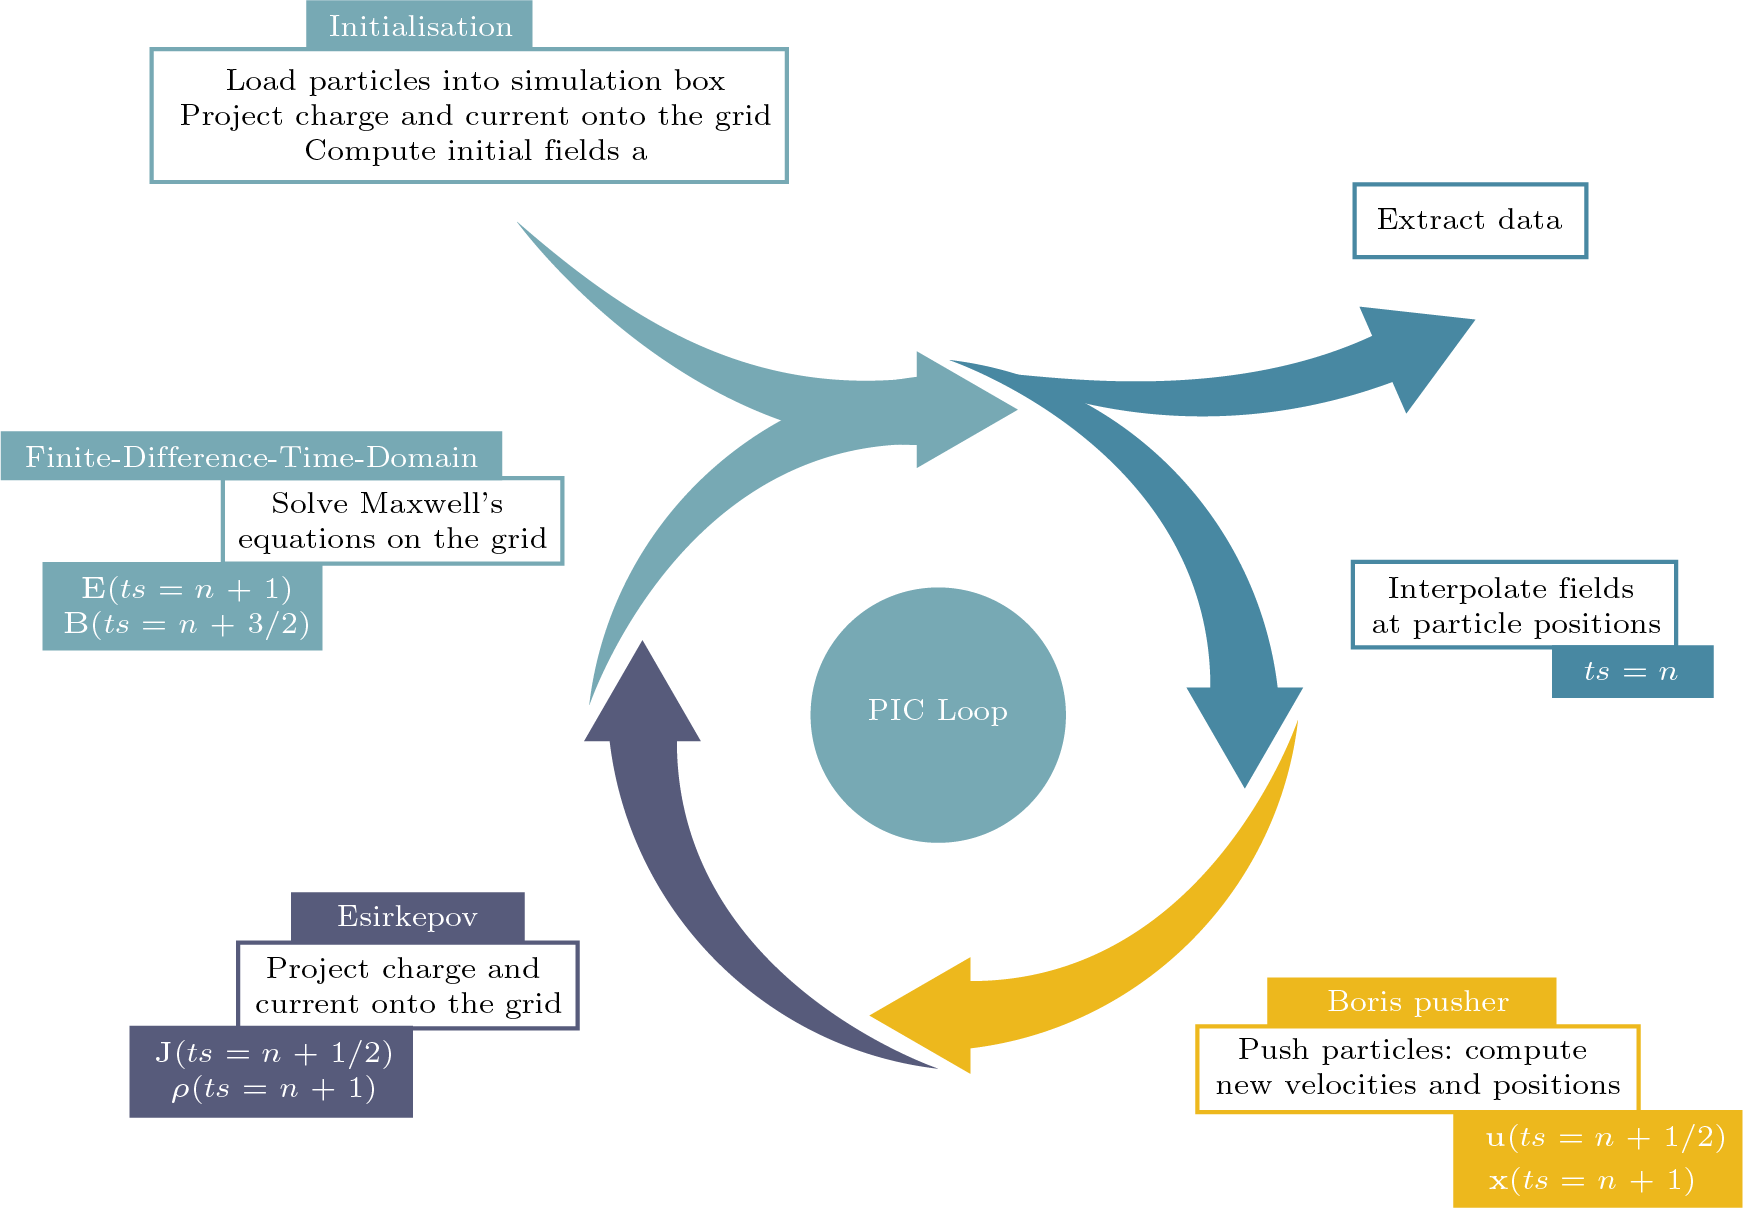
\includegraphics[width=\linewidth]{figures/intro/intro_PIC_cycle}
	\caption[A schematic of the PIC code loop and the algorithms performed.]{A schematic of the PIC code loop and the algorithms performed from time step, $ts$, from $n$ to $n+1$.}
	\label{fig:intropiccycle-01}
\end{figure}
After particle and field initialisation, fields are interpolated at particle positions. The well-established momentum-conserving \textit{Boris pusher} algorithm computes the new macro-particle velocities and positions \cite{borisRelativisticPlasmaSimulationoptimization1970}. Particles are advanced in time using a \textit{leap-frog }scheme, where positions are defined at integer, $n$, time steps and momenta at half-integer, $n + 1/2$. The charge conserving Esirkepov algorithm \cite{esirkepovExactChargeConservation2001} projects the new charge and current densities onto the grid to then solve Maxwell's equations on the grid using the Finite-Difference-Time-Domain approach \cite{tafloveComputationalElectromagneticsFiniteDifference2005}. To ensure space and time centring of the electromagnetic field derivatives in Maxwell's equations, electric and magnetic fields are discretised on the staggered \textit{Yee grid} as represented in figure \ref{fig:introyeegrid}. 
\begin{figure}
	\centering
	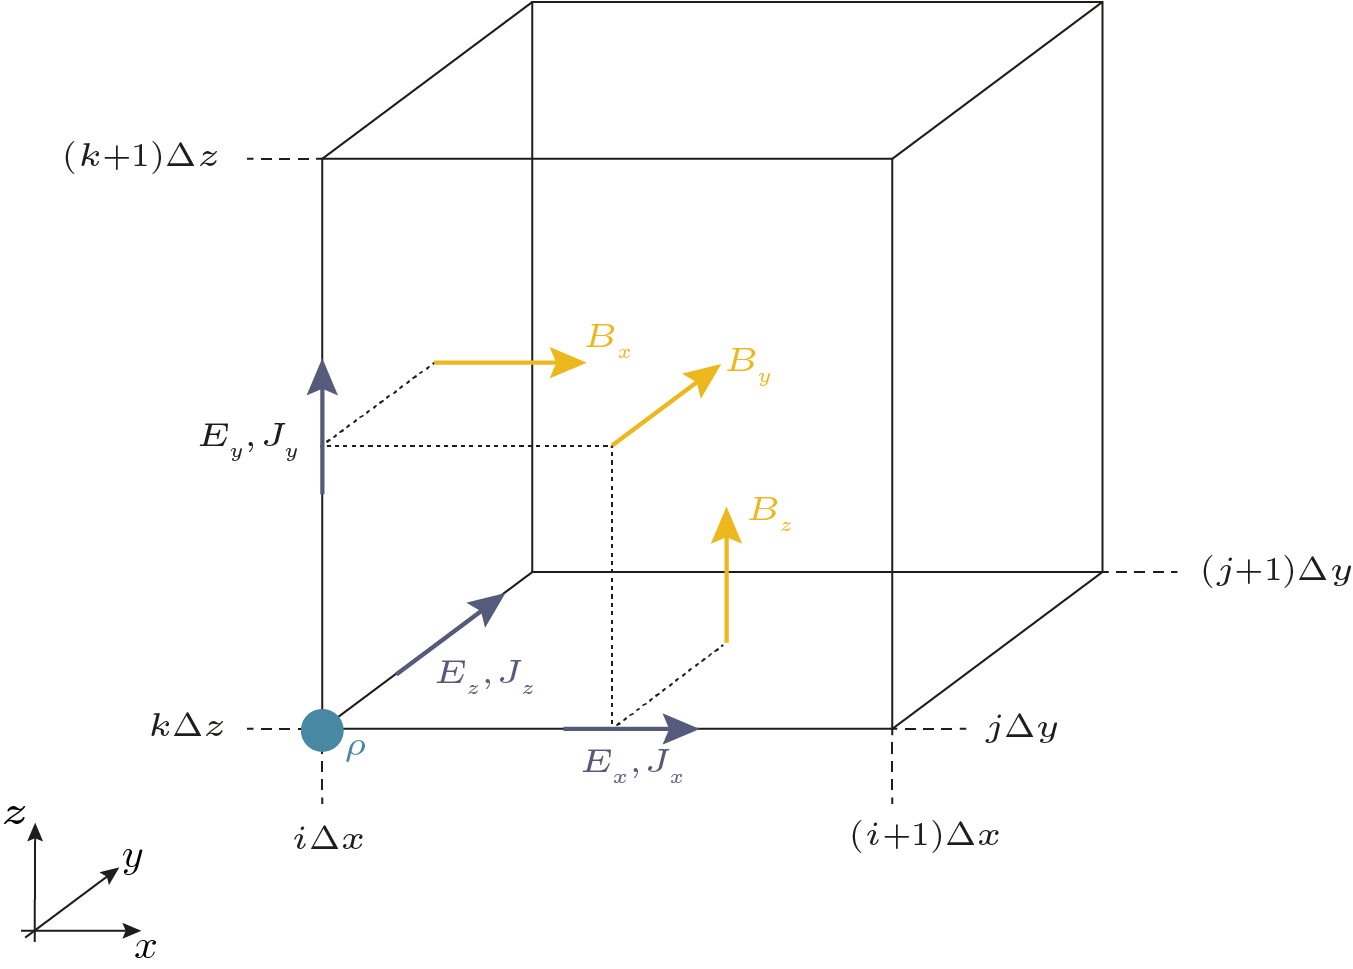
\includegraphics[width=0.7\linewidth]{figures/intro/intro_yee_grid}
	\caption[A representation of the staggered Yee grid.]{A representation of the staggered 3D Yee grid for the cell at $(i\Delta x, j\Delta y, k\Delta z)$ for spatial centring of the curl operations, including the locations where all system properties are defined.}
	\label{fig:introyeegrid}
\end{figure}
with electric fields defined at integer time steps and magnetic fields at half-integer time steps.

\subsubsection{Smilei}
Smilei (for Simulating Matter Irradiated by Light at Extreme Intensities) is a modern collaborative, massively parallel, fully relativistic and open source plasma physics PIC code and the major workhorse for this thesis\footnote{At points benchmarks against the EPOCH and Osiris PIC codes were performed.}. Produced by M. Grech's team(CHECK THIS) at École Polytechnique \cite{derouillatSmileiCollaborativeOpensource2018}, its recent development was motivated by the rapid advancements of multi-petawatt facilities both globally and locally with the recent completion of the 10 PW Apollon laser facility and by the availability of supercomputing power which has `skyrocketed' in recent years \cite{derouillatSmileiCollaborativeOpensource2018}. Indeed, the 3D \ac{PIC} simulations discussed in this thesis required the parallelisation of almost 20 \% of the computing resources available on ARCHER2.

\subsubsection{Reference units}
Given the broad range of magnitudes linked to multi-petawatt and femtosecond laser pulses, solid density plasmas, micrometre wavelengths, and attosecond electron bunches, it becomes significantly more convenient to transform them into dimensionless normalised values. Smilei operates in such units. This normalisation is not chosen \textit{a priori}, instead results can be scaled by an arbitrary reference angular frequency. This is extremely useful when working with boosted frames of reference. As this thesis focuses on the interaction of a laser pulse with plasma, the laser pulse angular frequency, $\omega_\mathrm{L}$ is set as the frequency of reference. A list of the most common normalisations is given in table \ref{tab:intro-normalisations}.

\begin{table}
	\begin{center}
		\begin{tabular}{ccc}
			\hline \hline
			Units of & SI units & Normalisation \\
			\hline
			velocity & \unit{m.s^{-1}} & $c$ \\
			charge & C & $e$ \\
			mass & kg & $m_\mathrm{e}$ \\
			momentum & \unit{kg.m.s^{-1}} & $m_\mathrm{e}c$ \\
			energy/temperature & J & $m_\mathrm{e}c^2$ \\
			time & s & $\omega^{-1}_\mathrm{L}$ \\
			length & m & $c/\omega_\mathrm{L}$ \\
			number density & \unit{m^{-3}} & $n_\mathrm{c}$ \\
			electric field & \unit{V.m^{-1}} & $m_\mathrm{e}c\omega_\mathrm{L}/e$ \\
			\hline \hline
		\end{tabular}
		\caption{\label{tab:intro-normalisations} Smilei normalisations for common quantities with the laser angular frequency $\omega_\mathrm{L}$ set at the reference angular frequency.}
	\end{center}
\end{table}

\subsubsection{Simulation parameters}\label{sec:intro-general_simulation_paramers}
\textit{Silver-M$\ddot{u}$ller} boundary conditions for the simulation box edges \cite{barucqAsymptoticBehaviorSolutions1997} are able to absorb and inject electromagnetic waves and particles. Note that there can be non-physical reflection of electromagnetic waves at such boundaries leading to some error.

The quasi-particle shape function $S(\mathbf{x})$ determines the projection of particle charge onto the grid. It is symmetric in all dimensions with respect to $\mathbf{x}$ and extends over $n$ cells of width $\Delta x$ in each direction where $n$ is the interpolation order. It can be written as a product across $D$ dimensions,
\begin{equation}
	S(\mathbf{x}) = \Pi^D_{\mu = 1}s^{(n)}(x^\mu).
\end{equation}
Smilei implements orders 2, 3 and 4, the explicit shape functions are
\begin{subequations}
	\begin{align}
		s^2 (n) &= \begin{cases}
			\frac{1}{\Delta x}\left(1-\left|\frac{x}{\Delta x}\right| \right)  & \text{if } |x| \le \Delta x, \\
			0  & \text{otherwise,}
		\end{cases} \\
		s^3(n) &= \begin{cases}
			\frac{3}{4\Delta x}\left(1-\frac{4}{3}\left(\frac{x}{\Delta x}\right)^2 \right)  & \text{if } |x| \le \frac{1}{2}\Delta x, \\
			\frac{9}{8\Delta x}\left(1-\frac{2}{3}\left|\frac{x}{\Delta x}\right| \right)^2  & \text{if } \frac{1}{2}\Delta x <|x| \le \frac{3}{2} \Delta x, \\
			0  & \text{otherwise,}
		\end{cases}  \\
		s^4(n) &= \begin{cases}
			\frac{2}{3 \Delta x}\left( 1-\frac{3}{2}\left(\frac{x}{\Delta x}\right)^2 + \frac{3}{4}\left| \frac{x}{\Delta x}\right| ^3 \right)  & \text{if } |x| \le \Delta x, \\
			\frac{4}{3 \Delta x}\left(1-\frac{1}{2}\left|\frac{x}{\Delta x}\right| ^3 \right)  & \text{if } \Delta x <|x| \le 2\Delta x, \\
			0  & \text{otherwise.}
		\end{cases} 
	\end{align}
\end{subequations}

While the correct implementation of collisions in PIC codes remains an open problem \cite{Collisions}, Smilei has implemented relativistic binary collisions between macroparticles using a Monte-Carlo-based scheme \cite{perezImprovedModelingRelativistic2012}. The aforementioned QED processes of Inverse Compton scattering and non-linear Breit-Wheeler pair production are included using the built-in Smilei packages \cite{derouillatSmileiCollaborativeOpensource2018}. These processes can lead to cascades of many particles being added to the simulations. Macroparticle merging can increase simulation efficiency and reduce the memory footprint. Smilei implements such a scheme, inspired by that designed by Vranic \textit{et al} \cite{vranicParticleMergingAlgorithm2015}, that is computationally efficient and conserves energy, momentum and charge within a cell. While Smilei contains modules to handle ionisation, with reference to figure \ref{fig:intro_lasersystems} these are deemed unnecessary for the laser intensities considered in this thesis.

\subsubsection{Parallelisation in practice}
In the following discussion, where differences in language occur, objects are given as their ARCHER2 (Smilei) names. The Smilei simulation box consists of a grid of cells as in figure \ref{fig:introsmileiparallelisation}.
\begin{figure}
	\centering
	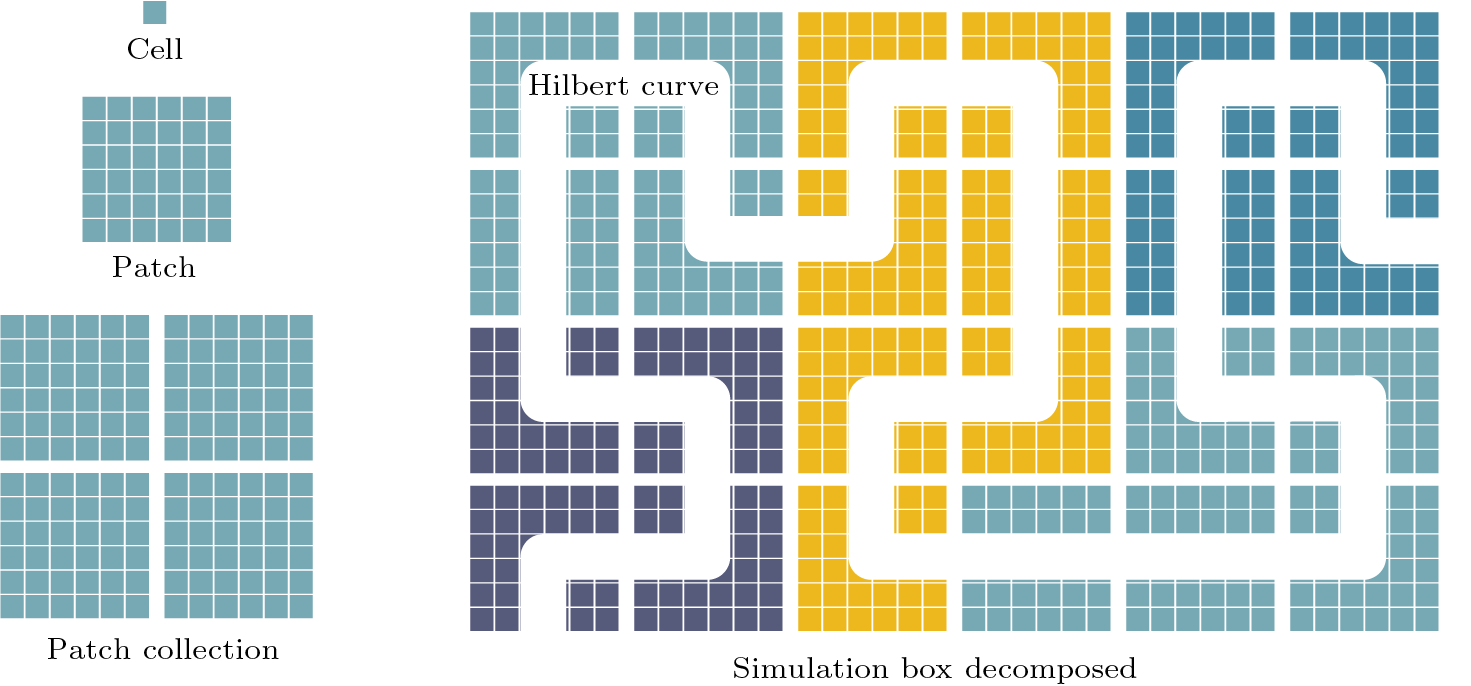
\includegraphics[width=1\linewidth]{figures/intro/intro_smilei_parallelisation}
	\caption[Smilei simulation box decomposition into cells, patches and MPI patch collections.]{Smilei simulation box decomposition into cells, patches and MPI patch collections. Cells are grouped into patches, patches are grouped into MPI patch collections. MPI patches are assigned contiguously along the Hilbert curve.}
	\label{fig:introsmileiparallelisation}
\end{figure}
The box is decomposed into \textit{patches} consisting of many cells. Patches are arranged into \textit{MPI patch collections} assigned contiguously along a Hilbert curve.

Archer consists of many \textit{CPUs (cores)} that can each perform computational tasks. CPUs are grouped into \textit{nodes}. Memory is shared within a node such that all CPUs (cores) in a node can operate on the same data. When optimised, ARCHER2’s memory in each node is split into 8 \textit{sockets}. These 8 sockets each perform a \textit{task (MPI process)}. Each task (MPI process) has 16 CPUs (cores) assigned that each perform a \textit{thread}. A thread is a sequence of instructions from the program.

Each task (MPI process) handles one \textit{MPI patch collection}. Threads work through patches. Figure \ref{fig:introsmileiparallelisationcomplex} represents this division of labour.
\begin{figure}
	\centering
	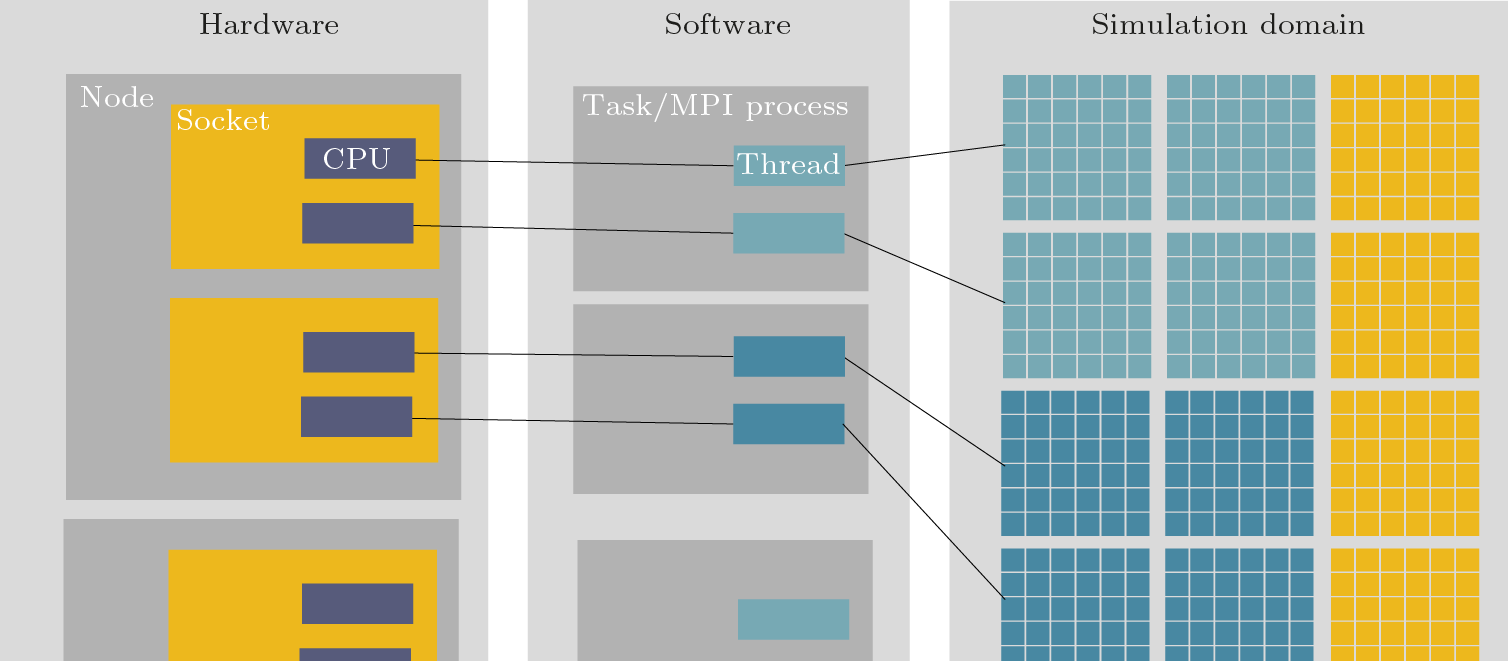
\includegraphics[width=1\linewidth]{figures/intro/intro_smilei_parallelisation_complex}
	\caption[Representation of the interaction of the ARCHER2 hardware and software components when running Smilei.]{Representation of the interaction of the ARCHER2 hardware and software components when running Smilei. Each CPU is assigned a thread, each task is carried out by one socket. A task tackles one MPI patch collection with threads working through patches.}
	\label{fig:introsmileiparallelisationcomplex}
\end{figure}
Threads do not need to wait for other threads in their process to tackle new patches in their MPI patch collection. This is a form of local \textit{dynamic load balancing}. If an MPI patch collection is overloaded, a patch is offloaded to a contiguous MPI patch collection.

There are several considerations for simulation optimisation. Tasks (MPI processes) should always be assigned more patches than threads. To apply the Hilbert curve, the number of patches in each dimension must be a power of 2. The fewer cells in a patch, the more efficient the load balancing, however, the cost of synchronisation between patches increases, although generally the gain in efficiency from load balancing by increasing patch number will win out at later times with increasing efficiency for increased frequency of load balancing \cite{derouillatSmileiCollaborativeOpensource2018}. Note that smaller patches are preferable when there are small regions with large numbers of particles, as in laser-solid surface interactions, however, the minimum patch size is dependent on the shape function of the macro-particles.

\subsubsection{Sources of error inherent to PIC codes}
Despite their relatively intuitive interpretation, PIC codes are famously finickety and prone to errors, most notably that of numerical self heating\footnote{Standard PIC code algorithms are charge and momentum conserving but not energy conserving \cite{derouillatSmileiCollaborativeOpensource2018}.}. There are three conditions required for stability.

To ensure stability, or at least to minimise instability, there are several conditions which must be met. Naturally, the time step, $\Delta t$, and cell size ($\Delta x$x$\Delta y$x$\Delta z$) must adequately capture all interesting features of a given simulation. Typically such features are plasma wave oscillations,
\begin{equation}
	\Delta t \omega_\mathrm{p} \ll 1,
\end{equation} 
and laser pulse electromagnetic field oscillations or higher order harmonics of the laser pulse if that is of interest, for the $n$th harmonic
\begin{equation}
	\Delta t\omega_\mathrm{L}n \ll 1.
\end{equation} 
Note this also ensures that macroparticles are smaller than the wavelengths of the system, a requirement to ensure they mimic real particles \cite{okudaCollisionsPlasmaFiniteSize1970}. Relativistic PIC codes must satisfy the much-acclaimed \cite{demouraCourantFriedrichsLewy2013} Courant-Friedrichs-Lewy condition,
\begin{equation}
	\frac{1}{c\Delta t} > \sqrt{\frac{1}{(\Delta x)^2}+\frac{1}{(\Delta y)^2}+\frac{1}{(\Delta z)^2}},
\end{equation}
thus preventing light and relativistic particles from crossing a cell in one timestep and generating numerical Cerenkov radiation \cite{birdsall2004plasma}. As with real plasmas and real particles, to avoid numerical charge fluctuation and ensure collective behaviour of macroparticles,
\begin{equation}
	\frac{4}{3}\pi\lambda_\mathrm{D}^3n_\mathrm{macro} = N_\mathrm{D,macro} \ggg 1,
\end{equation}
where $n_\mathrm{macro}$ is the macroparticle density \cite{birdsall2004plasma}. To avoid numerical heating, the cell size must resolve the Debye length,
\begin{equation}
	\frac{\lambda_\mathrm{D}}{\Delta x} \ge 1,
\end{equation}
failure to do so may cause plasma self-heating until the Debye length matches the cell size \cite{birdsall2004plasma}. Interestingly, Brackbill \textit{et al} \cite{brackbillEnergyMomentumConservation2016} observed in their simulations that setting $\lambda_\mathrm{D}/\Delta x =1$ was most effective at reducing spurious heating. Arber \textit{et al} \cite{arberContemporaryParticleincellApproach2015} performed extensive simulations exploring this instability. If the Debye length is not resolved, after an initial period of rapid self-heating, the temperature increases linearly and can be modelled as
\begin{equation}\label{eq:intro-selfheating}
	\frac{\mathrm{d} T_\mathrm{eV}}{\mathrm{d}t_\mathrm{ps}} = \alpha_\mathrm{H} \frac{n^{3/2}_{23} \Delta x^2_\mathrm{nm}}{N_\mathrm{ppc}},
\end{equation}
where $T_\mathrm{eV}$ is the temperature in electron volts, $t_\mathrm{ps}$ is the time in picoseconds, $n$ is the plasma electron number density in units of $10^{23}$ \unit{cm^{-3}}, $\Delta x_\mathrm{nm}$ is the cell size in nanometres and $N_\mathrm{ppc}$ is the number of macroparticles per cell with $\alpha_\mathrm{H}$, the heating coefficient, determined from their simulations. For a top-hat macroparticle shape function, they found $\alpha_\mathrm{H} = 3000$ with an order of magnitude reduction for every increase in order of the shape function and further improvements from using current smoothing techniques. Note that the heating curves are roughly self-similar at all points and thus while equation \ref{eq:intro-selfheating} was established in the linear regime only, its scalings remain useful to compare simulations at all times.

The final instability that shall be discussed is the \textit{finite grid instability}. This is the aliasing error associated with particle properties being deposited at grid points. Is most catastrophic for cold drifting plasmas and depends on the \textit{beam Debye length},
\begin{equation}
	B = \frac{u}{\omega_p \Delta x},
\end{equation}
where $u$ is the beam speed. While their theory predicts stability for $B > 0.25$, Brackbill \textit{et al} \cite{brackbillEnergyMomentumConservation2016} observed instability growth for all beam temperatures in their simulations, although they found the percentage error is a small fraction for $B>10$.

\subsection{Hydrodynamic codes}
A hydrodynamic code approximates the plasma distribution as a fluid. This is achieved by taking the moments of velocity of the distribution function, $f_s$ for fluid species $s$. The first three return the number density of particles
\begin{equation}
	n_s = \int f_s \mathrm{d}\mathbf{v},
\end{equation}
the fluid velocity, $\mathbf{u}_s$ and momentum,
\begin{equation}
	\mathbf{p_s} = m_sn_s\mathbf{u}_s = \int f_s \mathbf{v)\mathrm{d}\mathbf{v},
	\end{equation}
	and the pressure tensor
	\begin{equation}
		P_s = m_s\int f_s (\mathbf{v}-\mathbf{u}_s)(\mathbf{v}-\mathbf{u}_s)\mathbf{v}.
	\end{equation}
	The fluid equations that govern the evolution of these quantities can be extracted from the Vlasov equation, Equation \ref{eq:intro-vlasov} by taking the appropriate moment. Correspondingly producing the continuity equation
	\begin{equation}
		\frac{\partial n_s}{\partial t} + \nabla \cdot (n_s \mathbf{u}_s) = 0,
	\end{equation}
	the equation of motion
	\begin{equation}
		m_sn_s\left(\frac{\partial \mathbf{u}_s}{\partial t} + (\mathbf{u}_s\cdot \nabla) \mathbf{u}_s \right) = q_sn_s(\mathbf{E}+\mathbf{u}_s \times \mathbf{B}) - \nabla \cdot P_s
	\end{equation}
	
	ADD ENERGY TRANSPORT.
	
	The reduction of dimensionality achieved through this approximation dramatically reduces computational cost. However, much of this thesis relies on the precise velocity distribution of particles, naturally such a code cannot model these phenomena and the primary tool is the PIC code.
	% TODO add fluid equations as in Rob's thesis
	In this thesis, HYADES is the code of choice. HYADES is a 1D three fluid (electrons, ions and radiation) radiative hydrodynamic code \cite{larsenHYADESPlasmaHydrodynamics1994}. The equations of mass and energy transport are solved in a Lagrangian coordinate system, \textit{i.e.}, unlike strictly Eulerian PIC codes, the mesh defining regions of the simulation moves with the plasma it describes.
	
	\section{Powering the interaction}
	Two experiments are discussed in this thesis, one performed on ORION, and one planned on GEMINI. Their typical beam parameters are presented in Table \ref{tab:laser_params}.
	\begin{table}[]
		\centering
		\begin{tabular}{lccc}
			\hline \hline
			Parameter                & \multicolumn{2}{c}{ORION} & GEMINI \\ 
			Beamlines                & SP1         & SP2         & N \& S  \\ \hline
			Power (PW)               & 0.5         & 1           & 0.5    \\
			Energy (J)               & 200         & 500         & 12     \\
			Wavelength (nm)          & 527         & 1053        & 800    \\
			Parabola, $f/\#$ & $f/3$        & $f/3$        & $f/2$      \\
			Focal spot FWHM ($\mu$m) & < 20        & < 10        & 2      \\
			Duration (fs)            & 500         & 500         & 40     \\
			Shot rate                & 5/day       & 5/day       & 3/min  \\
			Peak $a_0$ (approx)      & 10          & 30          & 24    \\ \hline \hline
		\end{tabular}
		\caption{The ORION and GEMINI petawatt class short pulse beamlines for comparison. The GEMINI North (N) and South (S) beamlines are equivalent.}
		\label{tab:laser_params}
	\end{table}
	The GEMINI-PW laser facility of the \ac{CLF} at Harwell Campus, Oxfordshire is a petawatt class facility consisting of two 30 fs beams, \ac{N} and \ac{S}, each delivering a maximum focused intensity of \qty{2e21}{W.cm^{-2}} at a repetition rate of 0.05 Hz. Such a high frequency of operation has led to a paradigm shift in high-power laser physics experimentation with the arrival of statistically significant results.
	
	The ORION SP1 is produced by passing the SP2 through two frequency doubling crystals creating two equivalent beamlets that are then overlaid at the target. The double beamlet structure at the near-field is imaged in Figure \ref{fig:oriondoublebeamletsnearfield}.
	\begin{figure}
		\centering
		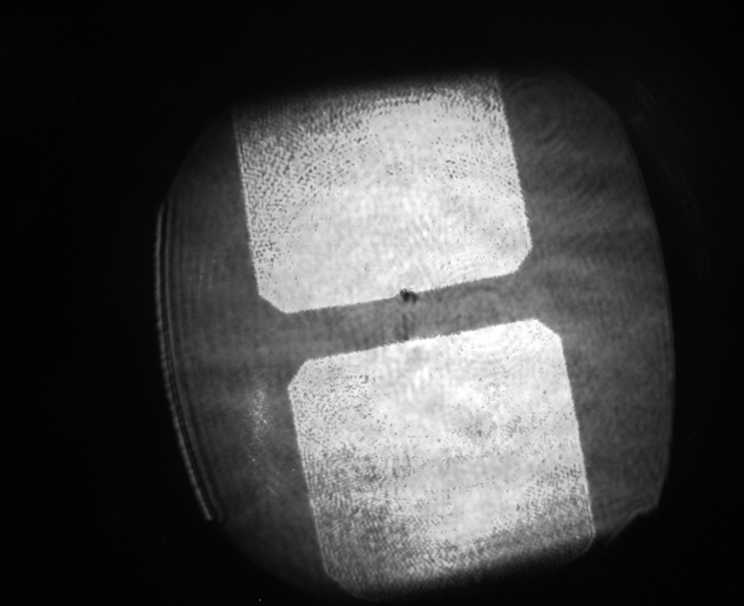
\includegraphics[width=0.5\linewidth]{figures/orion/orion_doublebeamlets_near_field}
		\caption[Image of the ORION SP1 double beamlet structure in the near-field.]{Image of the ORION SP1 double beamlet structure in the near-field. The two beamlets are then superimposed on the target.}
		\label{fig:oriondoublebeamletsnearfield}
	\end{figure}
	
	The ORION SP2 beamline intensity temporal profile can be modelled as
	\begin{equation}\label{eq:orion_SP2_temporal}
		I_\mathrm{SP2} \sim (I_{0 \ \mathrm{p}}\sech(t/t_\mathrm{p})^2 + I_{0 \ \mathrm{pp}}e^{-(t/t_\mathrm{pp})^2} + I_{0 \ \mathrm{ps}}e^{-\mathrm{abs}(t)/t_\mathrm{ps}} + I_{0 \ \mathrm{ns}}e^{-(t/t_\mathrm{ns})^8}),
	\end{equation}
	where the constants are detailed in Table \ref{tab:orion_pedestals} \cite{dhillierModelORIONContrast2022}.
	\begin{table}[]
		\centering
		\begin{tabular}{lcc}
			\hline\hline
			Pedestal, $i$                & $I_{0 \ i}$ & $t_i$  \\ \hline
			Main pulse, p                & 1           & 0.2 ps \\
			Picosecond pump residual, pp & $10^{-3}$   & 3 ps   \\
			Picosecond pedestal, ps      & \num{5e-5}  & 8 ps   \\
			Nanosecond pedestal, ns      & $10^{-11}$  & 3 ns  \\ \hline \hline
		\end{tabular}
		\caption{The native ORION SP2 pulse and prepulse pedestal constants as defined in Equation \ref{eq:orion_SP2_temporal}.}
		\label{tab:orion_pedestals}
	\end{table}
	The picosecond pump residual arises from parametric fluorescence in the ps OPA, the picosecond pedestal from scatter in the stretchers and noise on the OPA pump laser and the nanosecond pedestal from parametric fluorescence from the nanosecond OPAs. 
	% TODO understand the above, perhaps add more comments
	The SP1 temporal intensity profile is
	\begin{equation}
		I_\mathrm{SP1} \sim (I_\mathrm{SP2}^2 + I_\mathrm{SP2} \times 10^{-8}).
	\end{equation}
	The second term is due to the limitations of the harmonic separation system. The frequency doubling mechanism is not 100 \% efficient, \textit{i.e.} some of SP2 beamline remains and must be filtered out. The main pulse of the GEMINI beamlines is more appropriately modelled as a Gaussian.
	% TODO add a plot of the Gemini contrast
	
	\subsection{Laser contrast}
	% TODO In here add details about laser contrast and PMs
	
	% TODO: \textbf{INTRO CONCLUSION}